% Template for peer-reviewed articles
\documentclass[convention,student-expo]{aesconf} % peer-reviewed / express-paper / e-brief / student-expo

% Graphics path
\graphicspath{{./}{figures/}}

% UTF-8 encoding is recommended but use one that works for you.
\usepackage[utf8]{inputenc}

% Highly recommended package for better looking text automatically.
\usepackage{microtype}

% Natbib is used for more control on citations. You can use other modern
% bibliography packages but please try to match the provided style.
\usepackage[numbers,square]{natbib}


% These are useful for different purposes.
\usepackage{booktabs}
\usepackage{color}
\usepackage{url}


% The full title of the paper
\title{AmbiScopeVFX - Ambisonic Sound Field Visualizer outputting 360$^\circ$ Video in DaVinci Resolve}

% Put the authors in order here. The number in brackets define the corresponding affiliation.
\author[1]{Filip Lewiński}

% Affiliations go here
\affil[1]{Gdańsk University of Technology, Faculty of Electronics, Telecommunications and Informatics}



% Correspondece should include the corresponding author's name and e-mail address
\correspondence{Filip Lewiński}{fillewinski@gmail.com}

% These are used for headers. Anything that fits is okay. Please use proper punctuation.

% If there are many authors, please use the form "First author et al."
\lastnames{Lewiński}

% Short title should describe your topic but not be too long.
\shorttitle{AmbiScopeVFX - Ambisonics Visualizer for VR}


\begin{document}


\twocolumn[
\maketitle % MANDATORY!

\begin{onecolabstract}
This paper presents an open source solution for integrating ambisonic audio visualization with 360$^\circ$ video, targeting immersive virtual reality (VR) content production. The proposed tool, implemented as a Fuse plugin within DaVinci Resolve’s Fusion module, overlays a real-time ambisonic sound field heatmap onto video footage. It receives spatial intensity data via the Open Sound Control (OSC) protocol, transmitted from the IEM EnergyVisualizer plugin. The visualization facilitates synchronization and spatial coherence between audio and visual layers during editing. 
\end{onecolabstract}
]

\section{Introduction}

Virtual Reality (VR) represents the forefront of multimedia technology, offering an unparalleled sense of immersion through the integration of visual, auditory, and interactive components. To achieve a coherent and believable user experience in VR, synchronization between 360$^\circ$ video and spatial audio is essential. While spherical video formats allow viewers to freely explore a scene visually, ambisonic audio enables a spatially accurate sound field that responds to the user's head orientation, creating a natural and dynamic auditory experience.

Ambisonics, a spatial audio format based on spherical harmonics, has become a standard in immersive media due to its flexibility and rotational properties \citep{zotter2019ambisonics}. Unlike traditional channel-based formats, ambisonics allows for encoding the full sound field independently of playback configuration, making it ideal for VR applications. At the same time, 360$^\circ$ video—mapped onto a sphere—provides a panoramic visual environment, which, when combined with spatial audio, forms the basis of an engaging immersive experience.

However, aligning and editing these two modalities remains a technical challenge. Tools for simultaneous visualization and spatial correlation of ambisonic intensity with 360$^\circ$ video are limited, often requiring manual and time-consuming workflows. This project addresses this gap by presenting a tool for real-time ambisonic sound field visualization, directly overlaid on 360$^\circ$ video within DaVinci Resolve.

The proposed solution provides editors and sound designers with immediate insight into the spatial distribution of sound, supporting both synchronization and creative decision-making in immersive content production. By leveraging the Open Sound Control (OSC) protocol and integrating existing ambisonic tools such as the IEM EnergyVisualizer, this work offers a streamlined and extensible approach to editing spatial audio in a VR context.

\section{Methods}

The developed tool enables the real-time visualization of an ambisonic sound field directly within 360$^\circ$ video footage. It is implemented as a custom Fuse plugin for the Fusion module in DaVinci Resolve, providing a flexible and scriptable environment for post-production workflows. The system is designed to support immersive audiovisual editing by superimposing spatial audio data onto the video timeline.

\subsection{System Architecture}

The tool operates as a client in a local Open Sound Control (OSC) communication setup. Ambisonic spatial intensity data is generated externally by the IEM EnergyVisualizer plugin, which samples the energy distribution of the sound field across the surface of a virtual sphere. These values are transmitted over UDP using the OSC protocol \citep{wright2005osc,osc_spec}.

A lightweight Python backend, using the \texttt{python-osc} library, receives OSC messages and parses the data into a format consumable by the DaVinci Resolve plugin. The backend operates as an OSC server and ensures a minimal-latency data stream from the audio engine to the video compositor.

\subsection{Visualization Engine}

The Lua-based Fuse plugin within DaVinci Resolve reads the processed spatial intensity values and maps them onto a 2D representation of the 360$^\circ$ video. The primary projection format used is equirectangular, allowing compatibility with most video editors and preview systems. Alternatively, the tool also supports Hammer-Aitoff projection, preserving relative surface area and minimizing distortion—especially useful for analytical tasks.

The plugin generates a dynamic heatmap by converting root mean square (RMS) sound intensity values into color gradients, overlaying them onto the video frame. Each update cycle reflects the instantaneous energy distribution of the sound field, providing real-time spatial feedback to the editor.

\subsection{Implementation Details}

The system is designed to be cross-platform and requires only minimal configuration. It relies on open-source technologies and standards:
\begin{itemize}
    \item \textbf{Lua} for implementing the visualization layer within DaVinci Resolve's Fusion engine.
    \item \textbf{Python} for handling OSC data streams and preprocessing.
    \item \textbf{OSC protocol} over UDP for low-latency communication.
    \item \textbf{IEM EnergyVisualizer} for upstream generation of ambisonic energy field data \citep{rudrich2019iem}.
\end{itemize}

The modular nature of the implementation allows the tool to be extended to support additional projections, data formats, or spatialization plugins.

\section{Results}

The implemented visualization tool was successfully integrated into DaVinci Resolve as a Fuse plugin and tested in a typical 360$^\circ$ video editing workflow. The system allowed real-time rendering of ambisonic energy data over video footage, received via the Open Sound Control (OSC) protocol.

\subsection{Visualization Output}

The plugin rendered spatial intensity heatmaps in two projection formats:
\begin{itemize}
    \item \textbf{Equirectangular}, commonly used for editing 360$^\circ$ content,
    \item \textbf{Hammer-Aitoff}, offering lower distortion and better surface area preservation.
\end{itemize}
Heatmaps updated in real time, responding to frame-synchronized OSC messages generated by the IEM EnergyVisualizer plugin.

\begin{figure}[t]
\begin{center}
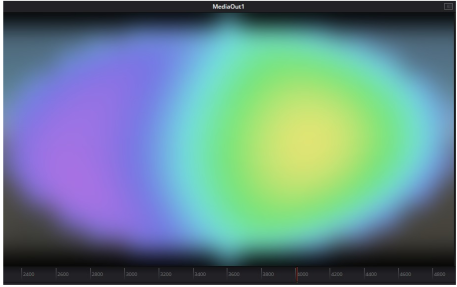
\includegraphics[width=0.95\columnwidth]{hammer-aitoff.png}
\caption{Example output of the plugin using the Hammer-Aitoff projection}
\label{fg:hammer_plot}
\end{center}
\end{figure}

\begin{figure}[t]
\begin{center}
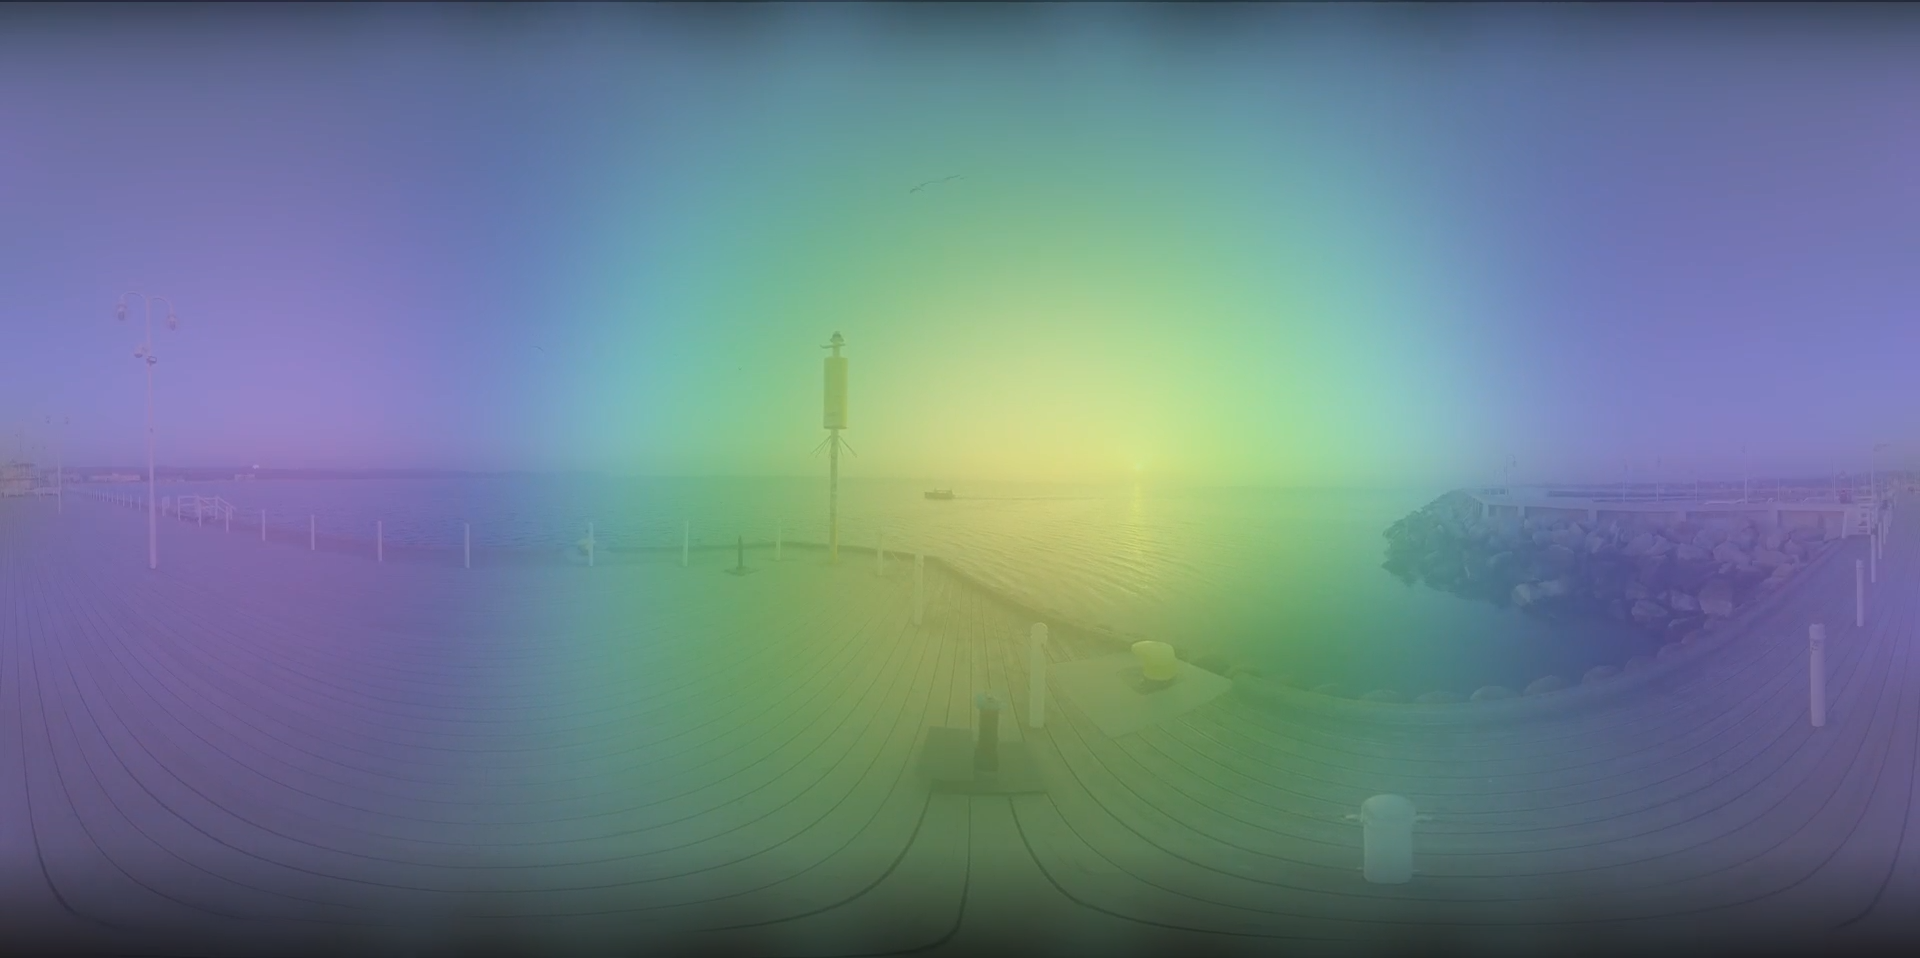
\includegraphics[width=0.95\columnwidth]{boat.png}
\caption{Example output of the plugin using the equirectangular projection with sample ambisonics and 360 video material.}
\label{fg:equirect_plot}
\end{center}
\end{figure}

\subsection{Compatibility and Constraints}

The tool currently supports OSC input structured according to IEM EnergyVisualizer's output format. The input coordinate system must be consistent with the projection mapping used by the plugin. Frame-level sync between audio analysis and video playback depends on both OSC update frequency and the editor’s timeline resolution.

\section{Discussion}

The results demonstrate that real-time ambisonic visualization is technically feasible within existing professional editing environments, using open protocols and customizable scripting layers. The system fills a gap in VR post-production workflows, where tools for spatial audio editing are often disconnected from the video timeline.

By overlaying a dynamic sound field heatmap directly onto 360$^\circ$ footage, the tool enhances editors’ ability to align auditory cues with visual content. This spatial awareness is especially valuable in immersive storytelling, where the coherence of multimodal information directly affects user presence and comfort \citep{yagunova2021ambisonics}.

Some observed limitations, such as the need for synchronized OSC updates and consistent spatial coordinate systems, are inherent to working with time-dependent spatial data. Future work could include buffering mechanisms for OSC input, or timeline-locked audio analysis baked into the editing session.

Beyond technical enhancements, the project raises questions about the role of visualization in spatial audio editing. While the heatmap provides intuitive feedback for spatial distribution, additional metrics—such as interactivity zones, listener focus estimation, or temporal diffusion patterns—could offer deeper insights during mixdown and design.

Overall, the tool’s successful deployment in a high-performance environment like DaVinci Resolve shows that spatial audio visualization can be brought closer to the editing process, empowering creators to refine immersive content with greater precision.

\section{Summary}

This work presented an open source tool for real-time visualization of ambisonic sound fields over 360$^\circ$ video, aimed at improving spatial awareness in VR content production. The system integrates the IEM EnergyVisualizer plugin with DaVinci Resolve via the OSC protocol and a custom Lua-based Fuse plugin. Testing confirmed that the visualization is responsive, projection-accurate, and introduces negligible performance overhead in a professional editing environment.

The approach enhances the creative workflow for immersive media by bridging spatial audio analysis with visual editing. While currently tailored to IEM’s data format, the architecture is modular and open to future extensions. Overall, the project demonstrates a practical method for supporting audiovisual coherence in VR storytelling, highlighting the growing importance of integrated tooling for immersive content development.

\bibliographystyle{jaes}

% Reference to bibliography file.
\bibliography{refs}

\end{document}
